\chapter{Register File}

\section{Cosa è?}
Il Register File è una memoria veloce all'interno della CPU che contiene registri utilizzati per memorizzare dati temporanei durante l'esecuzione delle istruzioni

\section{Da cosa è composto?}
Ogni registro è costituito da:
\begin{itemize}
    \item \textbf{D Flip-Flop}: Per memorizzare ogni singolo bit
    \item \textbf{Multiplexer}: Per selezionare quale registro leggere o scrivere
    \item \textbf{Decoder}: Per indirizzare correttamente i registri
    \item \textbf{Circuiti di controllo}: Per gestire lettura/scrittura sincronizzate con il clock
\end{itemize}

\begin{minipage}[t]{0.45\textwidth}
    \subsection{Schema}
    \begin{center}
        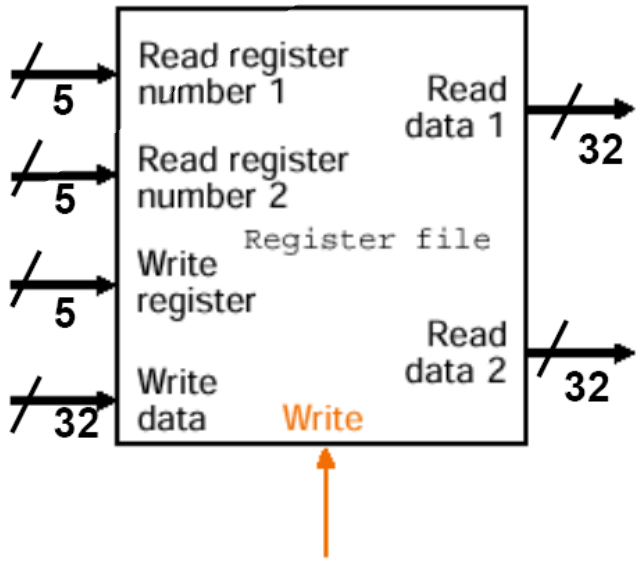
\includegraphics[scale=0.3]{Immagini/Register File.png}
    \end{center}
\end{minipage}
\hfil
\begin{minipage}[t]{0.45\textwidth}
    \subsection{Spiegazione porte}
    
    \subsubsection{Registri in lettura}
    \begin{itemize}
        \item \textbf{Read Reg1 (5 bit)}
        \begin{itemize}
            \item Numero del 1° registro da leggere
        \end{itemize}

        \item \textbf{Read Reg2 (5 bit)}
        \begin{itemize}
            \item Numero del 2° registro da leggere
        \end{itemize}

        \item \textbf{Read data 1 (32 bit)}
        \begin{itemize}
            \item Valore del 1° registro, letto sulla base di Read Reg1
        \end{itemize}

        \item \textbf{Read data 2 (32 bit)}
        \begin{itemize}
            \item Valore del 2° registro, letto sulla base di Read Reg2
        \end{itemize}
    \end{itemize}

    \subsubsection{Registri in scrittura}
    \begin{itemize}
        \item \textbf{Write Reg \# (5 bit)}
        \begin{itemize}
            \item Numero del registro da scrivere
        \end{itemize}

        \item \textbf{Write data (32 bit)}
        \begin{itemize}
            \item Valore da scrivere nel registro Write Reg \#
        \end{itemize}
    \end{itemize}

    \subsubsection{Segnali di controllo}
    \begin{itemize}
        \item \textbf{Write}
        \begin{itemize}
            \item Segnale di controllo messo in AND con il clock
            \item Solo se \texttt{Write=1}, il valore di Write data viene scritto in uno dei registri
        \end{itemize}
    \end{itemize}
\end{minipage}


\section{Lettura dal Register File}
\begin{minipage}[t]{0.45\textwidth}
    \subsection{Schema}
    \begin{center}
        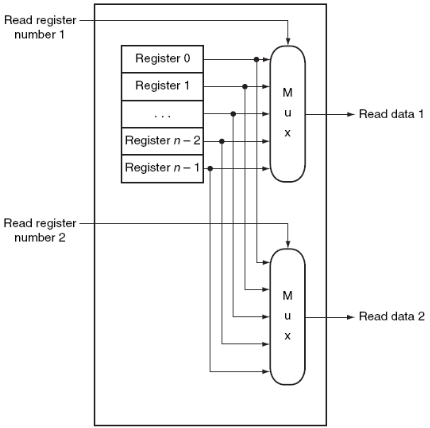
\includegraphics[scale=0.6]{Immagini/Lettura Register File.png}
    \end{center}
\end{minipage}
\hfil
\begin{minipage}[t]{0.45\textwidth}
    \subsection{Spiegazione}
    \begin{itemize}
        \item Utilizza 2 segnali che indicano i registri da leggere
        \item Utilizza 2 multiplexer: ognuno con 32 ingressi e un segnale di controllo
        \item Il register file fornisce sempre in output una coppia di registri
    \end{itemize}
\end{minipage}

\newpage
\section{Scrittura nel Register File}

\subsection{Schema}
\begin{center}
    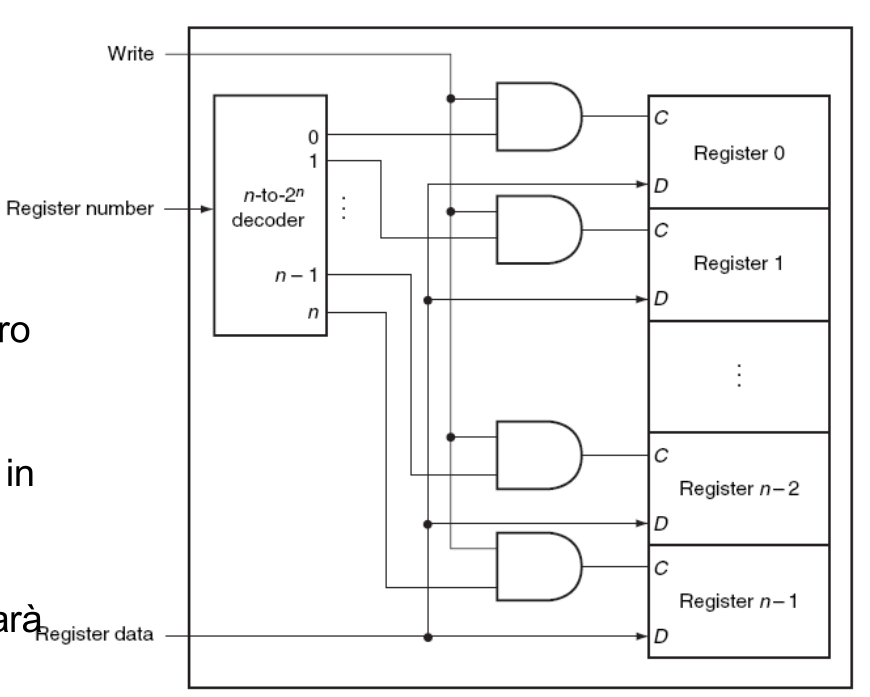
\includegraphics[scale=0.5]{Immagini/Scrittura Register File.png}
\end{center}

\subsection{Spiegazione}
\begin{itemize}
    \item Utilizza 3 segnali:
    \begin{itemize}
        \item Il registro da scrivere (Register Number)
        \item Il valore da scrivere (Register Data)
        \item Il segnale di controllo (Write)
    \end{itemize}

    \item Utilizza un decoder che decodfica il numero del registro da scrivere (Write Register)
    
    \item Il segnale Write (già un AND con il clock) è in AND con l'output del decoder
    
    \item Se Write non è affermato nessun valore sarà scritto nel registro
\end{itemize}